\chapter{Novel Approaches}

\subsection{Short Factors}
Searching for a decomposition using only the maximal divisors of $|Q|$, provides good solutions in \LogSpace, but there are certain limitations. Consider for example figure \ref{fig:shor/t-factors} depicting the trivial \DFA $A$ with its factors $A_2$ and $A_4$. Since for this \DFA, $|Q| = 8$, the only maximal divisor is 4 so the factor $A_4$ will be found be the original algorithm. In this particular example, there exists a smaller factor with size 2, $A_2$ which will only be found if checking all factors of $|Q|$ instead of only the maximal divisors.

\begin{figure}[h]
	\begin{minipage}[t]{\textwidth}
		\centering
		\begin{tikzpicture}[shorten >=1pt,node distance=1.5cm,on grid,auto] 
			\node[state,initial] (q_0)   {$q_0$}; 
			\node[state,accepting] (q_1) [ right=of q_0] {$q_1$}; 
			\node[state] (q_2) [ right=of q_1] {$q_2$}; 
			\node[state,accepting] (q_3) [ right=of q_2] {$q_3$};
			\node[state](q_4) [ right=of q_3] {$q_4$};
			\node[state,accepting] (q_5) [ right=of q_4] {$q_5$};
			\node[state] (q_6) [ right=of q_5] {$q_6$};
			\node[state,accepting] (q_7) [ right=of q_6] {$q_7$};
			\path[->] 
			(q_0) edge  node {} (q_1)
			(q_1) edge  node {} (q_2)
			(q_2) edge  node {} (q_3)
			(q_3) edge  node {} (q_4)
			(q_4) edge  node {} (q_5)
			(q_5) edge  node {} (q_6)
			(q_6) edge  node {} (q_7)
			(q_7) edge[bend right, above]  node {} (q_0);
		\end{tikzpicture}		
	\end{minipage}
	\begin{minipage}[b]{0.39\textwidth}
		\centering
		\begin{tikzpicture}[shorten >=1pt,node distance=1.5cm,on grid,auto] 
			\node[state,initial] (q_0)   {$q_0$}; 
			\node[state,accepting] (q_1) [right=of q_0] {$q_1$}; 
			\path[->] 
			(q_0) edge  node {} (q_1)
			(q_1) edge[bend right, above]  node {} (q_0);
		\end{tikzpicture}
	\end{minipage}
	\begin{minipage}[b]{0.59\textwidth}
		\centering
		\begin{tikzpicture}[shorten >=1pt,node distance=1.5cm,on grid,auto] 
			\node[state,initial] (q_0)   {$q_0$}; 
			\node[state,accepting] (q_1) [right=of q_0] {$q_1$}; 
			\node[state](q_2) [right=of q_1] {$q_2$};
			\node[state,accepting](q_3) [right=of q_2] {$q_3$};
			\path[->] 
			(q_0) edge  node {} (q_1)
			(q_1) edge  node {} (q_2)
			(q_2) edge  node {} (q_3)
			(q_3) edge[bend right, above]  node {} (q_0);
		\end{tikzpicture}
	\end{minipage}
	\caption{The DFA $A$ and its factors $A_4$ \& $A_2$}
	\label{fig:short-factors}
\end{figure}

TODO: Complexity if all divisors are used instead of maximal divisors

Given a positive integer $n$, let $d(n)$ denote the number of divisors of $n$ including 1 and $n$, so for example $d(8)=4$. More generally, if $n$ has a prime factorization $n = p_1^{a_1} \ldots p_k^{a_k}$ then by the fundamental theorem of arithmetic $d(n) = (a_1+1) \ldots (a_k+1)$. Clearly, $d(n) \leq n$ and therefore $d(n) = n^{o(1)}$.  


\subsection{Fourier Transform}
TODO: describe idea

\section{Modified Decomposition Problem}
The original problem was solvable in \LogSpace, but extending the problem to e.g. the Fourier-transformed factors, we face a different problem. Finding all the factors is fast but choosing which factors are actually required in the decomposition, is not. This problem can be described as:

Given an input $u = 101101\dots$ as binary word, and integer $k$ and the set of found factors $w_1, w_2, \dots, w_n$ with $l(u) > l(w_n) ~\forall n$ and $\#1(w_n) = 1 ~\forall n$. Find indices $i_1, i_2 \dots i_k$ such that
\[
\underbrace{w_{i_1}, w_{i_1}, \dots, w_{i_1}}_{l(u)} \cup_k = u
\]

To reduce the problem you described to the Set Cover problem, we'll create a Set Cover instance as follows. The universe $U$ will consist of all possible $k$-length binary words that can be formed. There are $2^k$ such words.
For each word $w_i$ in the given set of words $w$, create a corresponding subset $C_i$ of $U$. This subset contains all $k$-length binary words that can be formed by choosing $k$ indices $i_1, i_2 \dots i_k$. The Set Cover problem now involves finding the minimum number of subsets from $C$ that cover the entire universe $U$. Now, the goal is to show that if we can efficiently solve the Set Cover problem for this constructed instance, we can efficiently solve the original problem.

If the Set Cover problem finds a cover of size $k$, it means there is a set of indices $i_1, i_2, \dots, i_k$ that chooses from the words $w_i$ such that $w_{i_1}, w_{i_2}, \dots, w_{i_k}$ can form the same binary word as $u$, which satisfies the original problem. Conversely, if you can efficiently solve the original problem and find a set of indices $i_1, i_2, \dots, i_k$ that chooses from the words $w_i$ to form $u$, then the corresponding subsets $C_i$ in the constructed Set Cover instance cover the entire universe $U$. This means you've found a Set Cover of size $k$. This reduction demonstrates that solving the original problem is at least as hard as solving the Set Cover problem. Therefore, if you can efficiently solve Set Cover, you can also efficiently solve the original problem, and vice versa.

\begin{figure}[h]
	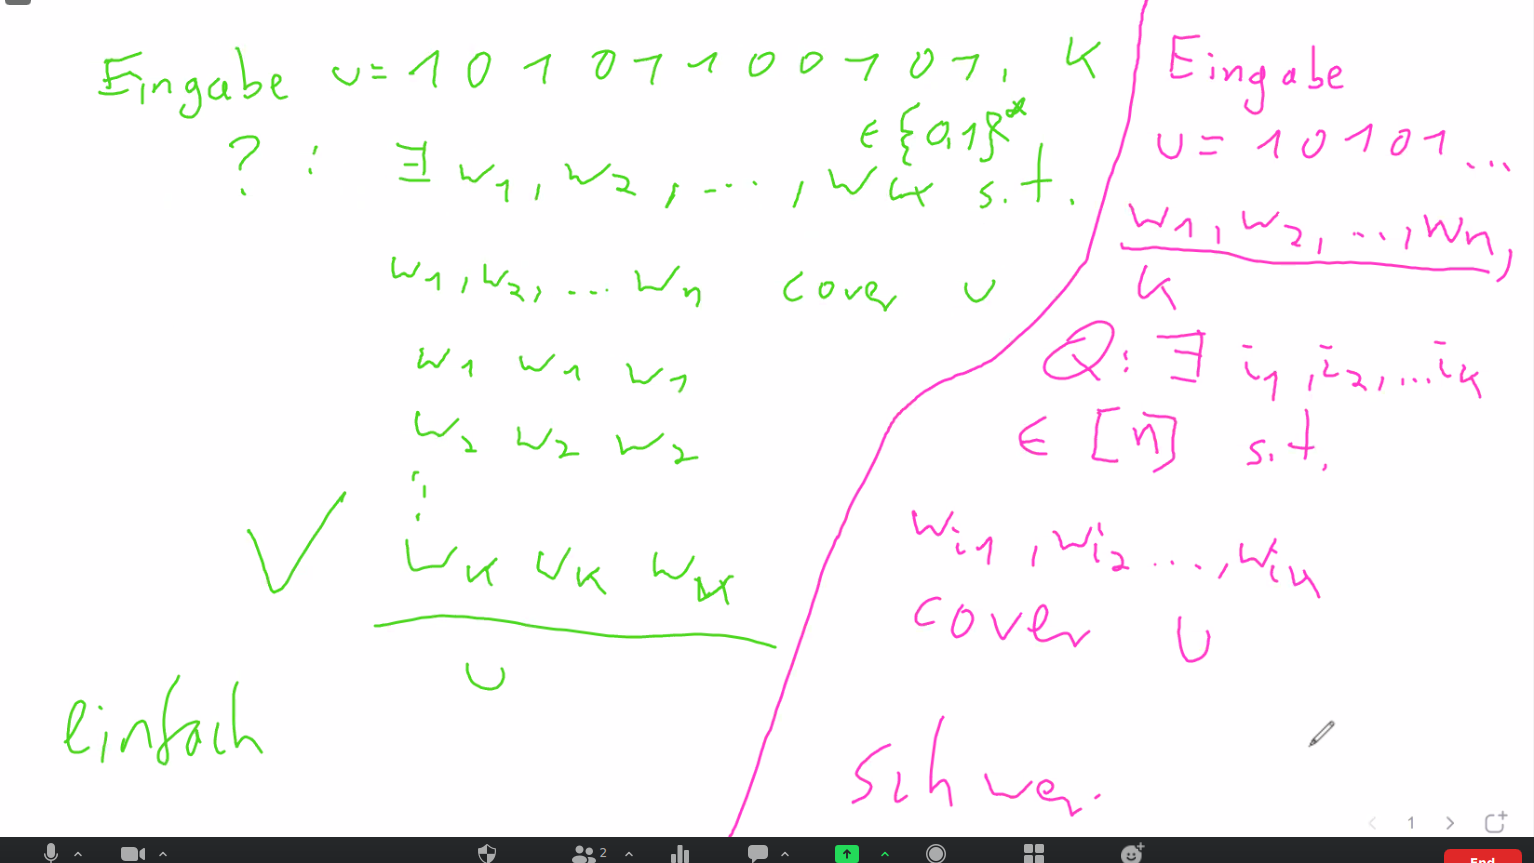
\includegraphics[width=\linewidth]{proof-sketches/Screenshot[2]-01.png}
\end{figure}